\chapter{Hardware implementeringen og operativ system}\label{kap:hardware}

\begin{figure}[h]
	\vspace*{-1 cm}
	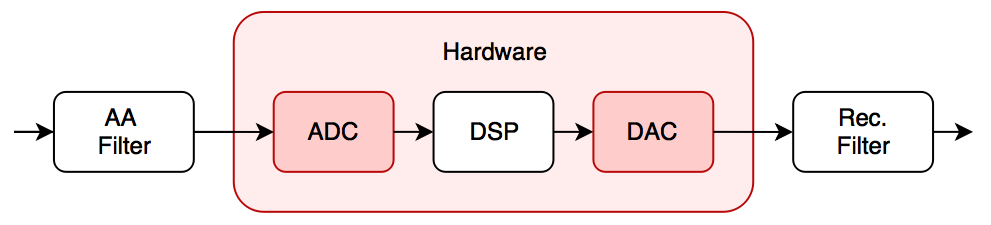
\includegraphics[width=7cm]{billeder/flow_hardware}
	\vspace{0.5 cm}
\end{figure}

I dette kapitel vil den komplette software og hardware løsning blive gennemgået som gør det muligt at udfører den digitale behandling af lydsignalet.
\husk{JJ}{Kort beskrivelse af de mellemliggende trin}
Til sidst vil der være en gennemgang af de nærliggende forbedringer og optimeringer.


\begin{enumerate}[noitemsep,nolistsep]
	\item Overblik af OS, lagdelt model
	\item Beskrivelse af Hardware lag - beskrivelse af de forskellige setups og hvorfor - fordele og ulæmper.
	\begin{enumerate}
		\item Initalisering af systemet som helhed - fastsættelse af beregningspunkter.
		\item Fastsættelse af clockfrekvens
		\item ADC
		\item LCD Driver 
		\item UART
		\item DAC / SPI
	\end{enumerate}
	\item håndtering af indgående lyssignal i de forskellige modes
	\item FPU math
	\item Schedulering af taskt - task model 
	\item Beskrivelse af de enkelte tasks
	\item Shell (ANSI / VT100) (Søren ?) 
	\item Quealizer profile model
	\item Debugging og task time profiling
	
\end{enumerate}






